% !TEX encoding = IsoLatin2  % notwendige Zeile f"ur Mac-Benutzer (muss als Kommentar stehen); Windows-Benutzer k"onnen die Zeile l"oschen.

% LaTeX-Vorlage Version 3.1,  Juli 2011
% erstellt von Dr. Andreas Drauschke (andreas.drauschke@technikum-wien.at) und Dr. Susanne Teschl (susanne.teschl@technikum-wien.at)
% geringf"ugig adaptiert von Harald Stockinger (harald.stockinger@technikum-wien.at)

 
\documentclass[a4paper,bibtotoc,oneside]{scrbook} 
% F"ur kurze Arbeiten w"are auch die Dokumentklasse "scrartcl" ausreichend. In diesem Fall ist "section" die h"ochste Ebene ("chapter" gibt es dann nicht).
% \documentclass[a4paper,bibtotoc,oneside]{scrartcl}

%\usepackage{cclicenses}

% verlinkte Querverweise im pdf
\usepackage{hyperref}

% deutsche Anpassungen
\usepackage[ansinew]{inputenc}
\usepackage[T1]{fontenc}
\usepackage[ngerman]{babel}

% mathematische Symbole
\usepackage{amsmath,amssymb,amsfonts,amstext}

% Kopfzeilen frei gestaltbar
\usepackage{fancyhdr}
\lfoot[\fancyplain{}{}]{\fancyplain{}{}}
\rfoot[\fancyplain{}{}]{\fancyplain{}{}}
\cfoot[\fancyplain{}{\footnotesize\thepage}]{\fancyplain{}{\footnotesize\thepage}}
\lhead[\fancyplain{}{\footnotesize\nouppercase\leftmark}]{\fancyplain{}{}}
\chead{}
\rhead[\fancyplain{}{}]{\fancyplain{}{\footnotesize\nouppercase\sc\leftmark}} 

% Farben im Dokument m"oglich
\usepackage{color}

% Schriftart Helvetica
\usepackage{helvet}
\renewcommand{\familydefault}{cmss} 

% Graphiken einbinden: hier f"ur pdflatex
\usepackage[pdftex]{graphicx}

\usepackage{array}

% H"ohe und Breite des Textk"orpers etwas gr"osser definieren
\setlength{\textheight}{225mm}
\setlength{\textwidth}{1.05\textwidth}

% weniger Warnungen wegen "uberf"ullter Boxen
\tolerance = 9999
\sloppy

% Anpassung einiger "Uberschriften 
\renewcommand\figurename{Abbildung}
\renewcommand\tablename{Tabelle}

\begin{document}

% Kopf- und Fusszeilen initiieren
\pagestyle{fancy}
\pagenumbering{Alph}

% Deckblatt:
\thispagestyle{empty}
\begin{picture}(0,0)
\color{white}\sffamily
\put(-101,-749){
\includegraphics[width=1.002\paperwidth, height=\paperheight]{BM_2011.pdf}}
\put(220,-670){
\includegraphics[width=0.5\textwidth]{FHTW_Logo_4c.pdf}}
\put(-30, -20){\bfseries\huge BACHELORARBEIT}
% Titel des Studienganges einf"ugen:
\put(-30,-50){\Large im Studiengang Bachelor Informatik}
% Titel der Arbeit einf"ugen:
% Die Minipage wird gesetzt, damit auch mehrzeilige Titel m"oglich werden.
\put(-32,-150){
\begin{minipage}{14cm}
\bfseries\huge Accessibility im Modern Web
\end{minipage}
}
% Name der Autorin/des Autors eingeben:
\put(-30,-250){\large Ausgef"uhrt von: Bernhard Posselt}
% Personenkennzeichen der Autorin/des Autors eingeben:
\put(-30,-270){\large Personenkennzeichen: 1010257029}
% Name der Begutachterin/des Begutachters eingeben:
\put(-30,-310){\large Begutachter: Dipl.-Ing. Mag. Dr. Michael Tesar}
\put(-30,-350){\large Wien, \today} % das Datum des letzten Kompilierens wird automatisch eingesetzt
\color{black}
\end{picture}

\newpage


\section*{Eidesstattliche Erkl"arung}\thispagestyle{empty}
\glqq Ich erkl"are hiermit an Eides statt, dass ich die vorliegende Arbeit selbst"andig angefertigt habe. 
Die aus fremden Quellen direkt oder indirekt "ubernommenen Gedanken sind als solche kenntlich gemacht. 
Die Arbeit wurde bisher weder in gleicher noch in "ahnlicher Form einer anderen Pr"ufungsbeh"orde vorgelegt
und auch noch nicht ver"offentlicht. Ich versichere, dass die abgegebene Version jener im Uploadtool entspricht.\grqq\\[5\baselineskip]
\rule{5cm}{0.2pt}\hfill\rule{5cm}{0.2pt}\\
\phantom{Datum }Ort, Datum\hfill Unterschrift\hspace{15mm}

\newpage


\section*{Kurzfassung}\thispagestyle{empty}
In dieser Arbeit wird ein "Uberblick "uber moderne Web-Technologien im Bereich
Accessibility gegeben. Immer mehr "offentliche Einrichtungen stellen im Rahmen des \emph{e-governments} heutzutage einen Zugang zu wichtigen Informationen und Services im Web bereit. Dadurch muss dieser Zugang universell erreichbar und nutzbar sein. Um eine L"osung f"ur dieses Problem zu finden, wird ein Blick auf die Empfehlungen der W3C geworfen. Auch auf neuere Techniken wie ARIA, die erst in einer \emph{Candidate Recommendation} vorhanden sind, wird eingegangen. Das Ziel dieser Arbeit ist, einen guten "Uberblick "uber den heutigen Stand der Accessibility im Web zu bieten und die Vorteile der Nutzung von Accessibility Methoden hervorzustreichen. 
\vfill
\paragraph*{Schlagw"orter:} Accessibility, Web, ARIA, HTML5


\newpage

\section*{Abstract}\thispagestyle{empty}
This thesis will present an overview over Accessibility techniques used in the
modern web. Over the last years, the usage of the web to present and
access information and services of public institutions has increased
dramatically. This requires services and information to be accessible for
every citizen. To find a solution for this problem, this thesis will look at
the W3C's recommendations and guidelines. Also newer techniques like ARIA
and the Role Attribute, which are currently in the \emph{Candidate Recommendation} phase, will be part of it. The goal of this thesis is to present the current status of Accessibility in the web and to show the advantages of using these techniques.
\vfill
\paragraph*{Keywords:} Accessibility, Web, ARIA, HTML5
\newpage

%\section*{Danksagung}
%\thispagestyle{empty}
%Text Text Text Text Text Text Text Text Text Text Text Text Text Text Text Text
%\newpage

\tableofcontents\thispagestyle{empty}
\newpage

\pagenumbering{arabic}
\setcounter{page}{1}

% Falls die Kapitel"uberschriften zu lang f"ur die Kopfzeile oder das Inhaltsverzeichnis sind, so erzielt man
% dort Kurzformen der Kapitelbezeichnungen mittels:
% \chapter[Kurzform]{Lange "Uberschrift}
\chapter{Einf"uhrung}
Das Web spielt im "offentlichen Bereich eine immer gr"o"sere Rolle: Viele
Services und Informationen werden bereits "uber eigens daf"ur erstellte Portale angeboten. Daraus folgt, dass das "offentliche Leben immer st"arker mit dem Web verwoben wird. Wie auch bei anderen "offentlichen Einrichtungen muss ein universeller Zugang f"ur alle B"urger erm"oglicht werden, auch f"ur jene, die mit k"orperlichen Einschr"ankungen oder Lernschwierigkeiten leben m"ussen, z. B. Blinde oder Personen mit eingeschr"ankten motorischen F"ahigkeiten. Solange dies nicht vollst"andig m"oglich ist, muss als Ersatz eine zus"atzliche Einrichtung bereitstehen, die "aquivalente M"oglichkeiten bietet \cite[S. 8]{understand_acc}. Es ist also auch im wirtschaftlichen Interesse "offentlicher Einrichtungen, ihre Services und Informationen barrierefrei anzubieten. 

Dadurch, dass diese Gruppe eine Minorit"at in der Bev"olkerung stellt und das Web auf oft mit speziellen Ein- oder Ausgabeger"aten verwendet - z. B. blinde Personen verwenden Screen-Reader oder Braillen - muss oft ein zus"atzlicher Aufwand bei der Erstellung von Webseiten betrieben werden. Ja "ofters wird sogar ganz darauf vergessen\cite[S. 7]{mod_software}. Roman Mauerhofer erfasst dieses Problem mit einem sehr treffenden Vergleich: \glqq Es ist beispielsweise so, als ob ein Architekt bei der Planung eines Bahnhofes den Einbau von Aufz"ugen vergisst.\grqq  \cite[S. 7]{mod_software}

Diese Gruppe macht jedoch keinen ganz so geringen Prozentanteil der Bev"olkerung aus wie "ofters angenommen. Laut einem Bericht des U.S. Census Bureau aus dem Jahre 2000 leben alleine in den USA ca. 49,7 Millionen Menschen mit k"orperlichen Einschr"ankungen und Lernschwierigkeiten (entspricht ca. 20\% der amerikanischen Bev"olkerung), davon haben 42,9 Millionen eine schwere Einschr"ankung und 6,8 Millionen haben eine so gravierende Einschr"ankung, dass sie Hilfe in ihrem allt"aglichem Leben brauchen \cite[S. 1]{us_cens}. Laut der \glqq World Health Organization\grqq wird der weltweite Anteil an Personen mit k"orperlichen Einschr"ankungen oder Lernschwierigkeiten auf 500 bis 600 Millionen Menschen gesch"atzt \cite{who_dis}.

Auch die UN erkennt eine immer gr"o"ser werdende Wichtigkeit bez"uglich einer angemessenen Bereitstellung von Informationen f"ur k"orperlich eingeschr"ankten Personen und Personen mit Lernschwierigkeiten. Dies spiegelt sich in der \glqq UN Convention of Rights for Persons with Disabilities\grqq wider, welche am 30. M"arz 2007 unterzeichnet wurde. Sie erhielt die \glqq meisten Unterschriften an einem Er"offnungstag in der Geschichte der UN Konventionen\grqq \cite{un_disabilities}. 

Jedoch kann es nicht nur aus den oben genannten Gr"unden erforderlich sein,
einen barrierefreien Zugang bereitzustellen, sondern es wird sogar oft gesetzlich vorgeschrieben. In den USA beispielsweise, gibt es daf"ur ein eigenes Gesetz, den \glqq Americans with Disabilities Act\grqq aus dem Jahre 1990 (ADA) und den Abschnitt 508 aus dem \glqq Rehabilitation Act\grqq (1973) \cite[S. 288-289]{achieving_web_acc}. Auch in Europa sind einige "ahnliche Regelungen vorhanden \cite[S. 7]{mod_software}, doch eines haben die Meisten gemeinsam: Sie basieren nahezu alle zu einem gro"sen Teil auf den Richtlinien der WAI (Web Accessibility Initiative), den WCAG (Web Content Accessibility Guidelines) \cite[S. 289]{achieving_web_acc} \cite[S. 7]{mod_software}.

\section{Problemstellung}
Nicht nur in der EU wird Accessibility k"unftig eine gr"o"sere Rolle spielen \cite[Abschnitt EU]{w3c_pol}, sondern auch in der Privatwirtschaft. F"ur viele ProgrammiererInnen stellt jedoch die Implementation und das Testen von Accessibility Techniken einen nicht zu untersch"atzenden Mehraufwand dar \cite[S. 27]{understand_acc} und dadurch werden ihnen, selbst wenn sie sie umsetzen wollen, oft Steine in den Weg gelegt. Dies erfolgt h"aufig in der Nennung nicht zu Ende gedachter Argumente wie \glqq Barrierefreiheit bringt keine Vorteile\grqq \cite[S. 28]{understand_acc} oder \glqq Behinderte geh"oren nicht zu unserer Zielgruppe\grqq \cite[S. 31]{understand_acc}.

Ein weiteres Problem ist die geringe Verbreitung der Standards. Dies wurde in einer globalen Studie der \emph{United Nations} aus dem Jahre 2006 festgestellt\cite{acc_report}: Nur drei von 100 getesteten Seiten erhielten die Bestnote \cite [S. 7]{acc_report}. Dies ist unter anderem auf ein Fehlen folgender Punkte zur"uckzuf"uhren \cite[S. 13]{tool_acc}: 

\begin{itemize}
\item \emph{Achtsamkeit}: Vergessen oder "Ubersehen von Fehlern und Problemen im Bereich Accessibility
\item \emph{Bildung}: Accessibility-Techniken sind unbekannt
\item \emph{Tool Support}: Techniken werden nicht von Programmierwerkzeugen unterst"utzt
\end{itemize}


\section{L"osungsansatz}
In dieser Bachelorarbeit soll ein genereller "Uberblick "uber die bestehenden und einsetzbaren Techniken gegeben werden, die hilfreich f"ur Verbesserungen im Bereich Accessibility im Modern Web sind. 

Dazu soll eine "Ubersicht "uber die vom W3C bereitgestellten Spezifikationen, den WCAG 1.0 \cite{wcag1}, WCAG 2.0 \cite{wcag2} und ARIA \cite{aria} gegeben werden und au"serdem soll auf die Unterschiede von WCAG 1.0 und WCAG 2.0 eingegangen werden.

Zus"atzlich wird kurz auf die verschiedenen Arten von Einschr"ankungen eingegangen und die Probleme und verwendeten Hilfsger"ate werden aufgezeigt.

\section{Aufbau}
In Kapitel 2 wird ein kurzer "Uberblick "uber die h"aufigsten Einschr"ankungen gegeben und erkl"art, welche assistiven Technologien verwendet werden k"onnen, um k"orperlich eingeschr"ankten Personen und Personen mit Lernschwierigkeiten beim Zugriff auf das Web zu helfen. Dies soll veranschaulichen, warum  Webseiten f"ur diese Ger"ate optimiert werden sollen.

In Kapitel 3 wird auf die Richtlinien des W3C, die WCAG, eingegangen und Entwicklung und Unterschiede zwischen der Version 1.0 und Version 2.0 betrachtet.

In Kapitel 4 wird ein Blick auf ARIA geworfen und Sinn und Einsatzzweck von \emph{Roles}, \emph{States} und \emph{Properties} erl"autert.

In Kapitel 5 wird eine Zusammenfassung der jetzigen Situation und ein Ausblick "uber kommende Richtlinien gegeben, welche sich derzeit noch im \emph{Draft Status} befinden.

\section{Begriffe}
Da der Begriff \glqq Menschen mit geistigen Behinderungen/Einschr"ankungen\grqq negativ behaftet ist, wird in dieser Arbeit stattdessen der Begriff \glqq Menschen mit Lernschwierigkeiten\grqq  verwendet. Dies ist gleich zu setzen mit den Abschnitten F70-F79 im ICD-10 \cite{icd10}. Dazu z"ahlen unter anderem Menschen mit Konzentrationsschw"achen.


Der Begriff \glqq Menschen mit k"orperliche Einschr"ankung\grqq wird synonym f"ur Personen verwendet, welche durch eine Verletzung, Nichtfunktion oder Amputation eines K"orperteiles Einschr"ankungen im t"aglichen Leben erfahren m"ussen. Dazu z"ahlen unter anderem Menschen mit Sehschw"achen oder Blindheit und Menschen mit einer Fehlbildung der Finger oder H"ande.

\chapter{Arten von k"orperlichen Einschr"ankungen oder Lernschwierigkeiten
 und assistive Technologien}

\section{Personen mit Sehschw"achen}
Die Anzahl blinder Personen allein in den USA wird auf eine Million Personen und weltweit auf 38 Millionen Personen gesch"atzt\cite[S. 1]{screen_read}.  Als offiziell blind gilt eine Person, wenn sie unter 2\% auf dem besseren der zwei Augen wahrnimmt \cite[S. 12]{understand_acc}. 

Jedoch umfasst diese Kategorie nicht nur blinde Personen, sondern auch Personen mit teilweisen Sehschw"achen: Nimmt eine Person auf dem besten Auge weniger als 30\% wahr, f"allt sie bereits unter diese Kategorie\cite[S. 12]{understand_acc}. In "Osterreich betr"agt die Anzahl der Personen mit Sehschw"achen rund 318.000 Personen, das entspricht 3,9\% der Bev"olkerung \cite[S. 13]{stat_austria}. Es wird gesch"atzt, dass weltweit mindestens sechs Millionen Personen von so schweren Sehschw"achen betroffen sind, dass f"ur sie die Nutzung eines Computerbildschirmes unm"oglich ist\cite[S. 249]{screen_read_frust}.

Personen mit Sehschw"achen haben die gr"o"sten Probleme nicht mit den Eingabeger"aten - die meisten Nutzer beherrschen das Tippen ohne auf die Tastatur zu schauen - sondern eher mit den Ausgabeger"aten. Die am meisten genutzten assistiven Technologien in diesem Umfeld sind Screen-Reader und Braillen (siehe \ref{Abb1}). Braillen und andere in Hardware umgesetzte Technologien sind jedoch meistens sehr teuer, da sie nur von einem geringen Prozentsatz der Bev"olkerung ben"otigt werden und deren Erlernung, beispielsweise die der Braillenschrift, aufw"andig und dementsprechend wenig verbreitet ist\cite[S. 249-250]{screen_read_frust}.
Zus"atzlich besteht die Braille aus vielen kleinen, mechanischen Teilen und ist deshalb besonders verschlei"sanf"allig \cite[S. 11]{barr_webd}.

\begin{figure}[braille]
\centering
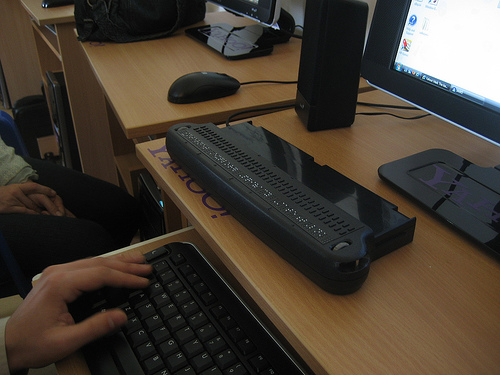
\includegraphics[width=75mm]{braille}
\caption[Beispiel einer Braille]{Beispiel einer Braille (\copyright  Philip Tellis, Creative Commons BY-SA)}\label{Abb1}
\end{figure}

Deshalb ziehen die Meisten auf Software basierende L"osungen vor, was dem Screen-Reader, etwa dem frei verf"ugbaren GNOME Orca \cite{orca}, zu einer h"oheren Popularit"at verhilft\cite[S. 249-250]{screen_read_frust}. Ein Screen-Reader liest dem/der NutzerIn die Inhalte auf dem Bildschirm vor. Dies kann f"ur sehende Personen als st"orend empfunden werden. Blinde Personen sind jedoch st"arker auf auditive Reize ausgerichtet und kommen dementsprechend besser damit klar\cite[S. 13]{barr_webd}. 

F"ur diese Personen muss beim Erstellen von Webseiten besonders Folgendes beachtet werden: semantisch korrekter und sauberer HTML Code, der den Inhalt vom Layout trennt.\cite[S. 13-15]{barr_webd}

\section{Personen mit H"orschw"achen}
Alleine in "Osterreich befinden sich ca. 202.000 Personen (2,5\% der Bev"olkerung) mit eingeschr"ankter H"orf"ahigkeit. Personen mit schweren H"orschw"achen machen rund 2.000 Personen aus \cite[S. 13-14]{stat_austria}. Die gr"o"sten Probleme entstehen f"ur diese Gruppe, wenn eine Webseite eine bestimmte Information nur "uber akustische Signale wiedergibt. Dies kann z. B. ein einfaches Video oder ein Podcast sein, oder ein Warnsignalton. \cite[S. 17]{barr_webd}\cite[S. 20]{understand_acc}

F"ur diese Personen muss vor allem Folgendes beachtet werden: Bereitstellung von Untertiteln bei Videos oder Transkriptionen von Podcasts und Verzichten auf \glqq audio-only\grqq L"osungen. Das Anbieten von Videos mit Geb"ardensprache kann n"utzlich sein, stellt jedoch einen hohen Aufwand dar, den jeder/jede AuftraggeberIn selbst f"ur sich entscheiden muss. \cite[S. 17]{barr_webd}\cite[S. 20]{understand_acc}

\section{Personen mit motorischen Schw"achen}
Diese Gruppe macht laut dem U.S. Census Report 21,2 Millionen Personen aus. Das
sind ca. 8,2 Prozent der Bev"olkerung der USA \cite[S. 1]{us_cens}. In "Osterreich betr"agt deren Anzahl 1 Million bzw. 13\% der Bev"olkerung \cite[S. 12]{stat_austria}. Probleme mit der Computerbenutzung treten vor allem dann auf, wenn Personen ihre H"ande nur eingeschr"ankt oder gar nicht verwenden k"onnen, beispielsweise Querschnittsgel"ahmte. F"ur diese muss eine alternative Steuerung des Computers angeboten werden. Darunter fallen z. B. Ger"ate, welche es den NutzerInnen erlauben, den Computer mit ihrer Zungenspitze zu bedienen.\cite[S. 15-16]{barr_webd}

Diese Art der Bedienung ist offensichtlich aufw"andiger und schwieriger und profitiert deshalb am meisten von einer klaren Struktur der Seite und einer guten Bedienbarkeit mit der Tastatur.\cite[S. 15-16]{barr_webd}\cite[S. 18]{understand_acc}

\section{Personen mit Lernschwierigkeiten}
Diese Gruppe macht laut dem U.S. Census Report 12,4 Millionen Personen aus. Das
sind ca. 4,8 Prozent der Bev"olkerung der USA \cite[S. 1]{us_cens}. Zu dieser Gruppe geh"oren auch Analphabeten, welche etwa in Deutschland ca. vier Millionen Personen ausmachen (ca. 6,3\% der deutschen Bev"olkerung) \cite[S. 19]{understand_acc}. In "Osterreich sind 85.000 Personen bzw. 1\% der Bev"olkerung von Lernschwierigkeiten betroffen \cite[S. 14]{stat_austria}.

Diese Personen haben vor allem Probleme mit zu komplizierten S"atzen oder einer fehlenden Struktur der Seite. Dadurch profitieren sie am meisten durch einfache und kurze S"atze, gute Strukturierung, den Einsatz von Bildern und einer M"oglichkeit, sich Texte vorzlessen zu lassen, auch \glqq Text-to-Speech\grqq genannt wird. \cite[S. 18-19]{barr_webd}\cite[S. 19]{understand_acc}

\chapter{WCAG}
Die WCAG (Web Content Accessibility Guidelines) ist ein Dokument, welches vom W3C herausgegeben wurde um Webseiten auch f"ur k"orperlich eingeschr"ankte Personen oder Personen mit Lernschwierigkeiten zug"anglich zu machen. 

Da sich viele Richtlinien mit der Optimierung des Inhaltes f"ur weniger gel"aufige Plattformen besch"aftigen, verbessert deren Anwendung auch die Plattformunabh"angigkeit. Dies kommt vor allem Ger"aten zu Gute, die durch Formfaktor oder Einsatzgebiet in Gr"o"se oder Funktion eingeschr"ankt sind, beispielsweise Mobiltelefonen. \cite[Abschnitt Abstract]{wcag1}


\section{WCAG Version 1.0}
Die Version 1.0 des Dokumentes wurde im Jahre 1999 finalisiert und beinhaltet 14 Richtlinien, welche jeweils Empfehlungen f"ur WebentwicklerInnen enthalten. Diese Empfehlungen enthalten Unterpunkte, so genannte Checkpoints, die wiederum mit einer Priorit"at gekennzeichnet sind. \cite[Abschnitt Abstract]{wcag1}

F"ur eine bessere Gegen"uberstellung dieser Kriterien mit denen der WCAG 2.0 wird versucht, diese 14 Richtlinien der WCAG 1.0 in die gleiche Struktur wie die der WCAG 2.0 zu bringen.

\subsection{Success Criteria}
Die Kriterien, anhand derer die erfolgreiche Umsetzung der Richtlinien gepr"uft werden k"onnen, werden in drei verschiedene Kategorien aufgeteilt: \emph{must}, \emph{should} und \emph{may} Kriterien, sprich Kriterien die erf"ullt sein m"ussen, sollten und k"onnen. Anhand der Erf"ullung dieser Kriterien lassen sich folgende Konformit"atslevel definieren: \cite[Abschnitt 4]{wcag1}

\begin{itemize}
\item \emph{A}: Alle mit Priorit"at 1 angef"uhrten Kriterien sind umgesetzt
\item \emph{AA}: Alle mit Priorit"at 1 und 2 angef"uhrten Kriterien sind umgesetzt
\item \emph{AAA}: Alle mit Priorit"at 1, 2 und 3 angef"uhrten Kriterien sind umgesetzt
\end{itemize}

Die deutsche BITV (Barrierefreie Informationstechnologie Verordnung), welche im \glqq Bundesgesetz zur Gleichstellung behinderter Menschen\grqq  festgeschrieben ist, baut z. B. auf diesen Kriterien auf. Sollen die BITV komplett erf"ullt werden, m"ussen sowohl die Kriterien der Stufe 1, als auch die der Stufe 2 komplett erf"ullt werden, was dem Konformit"atslevel AA entspricht. \cite[S. 38-39]{barr_webd}

\subsection{Wahrnehmbarkeit}
Unter die Kategorie Wahrnehmbarkeit fallen folgende Richtlinien: 

\begin{itemize}
\item Visuelle oder auditive Elemente sollten eine textbasierte Alternative besitzen\cite[Abschnitt 6.1]{wcag1}
\item Der Sinn des Inhalts sollte nicht nur von der Farbe abh"angig sein \cite[Abschnitt 6.2]{wcag1}
\end{itemize}

\subsubsection{Visuelle oder auditive Elemente sollten eine textbasierte Alternative besitzen}
Diese Richtlinie bezieht sich vor allem auf Personen mit Sehschw"achen und besagt, dass f"ur alle eingesetzten visuellen oder auditiven Elemente wie Bilder, Videos oder Kl"ange eine dementsprechende Alternative vorhanden sein sollte. Dies kann z. B. erreicht werden, indem \emph{<img>} Elemente immer ein \emph{alt} Attribut mit der Beschreibung des Bildes besitzen, oder Videos/Kl"ange mit einem beschreibenden Text oder Transkription versehen sind. Von den Kriterien, die  zur Erf"ullung dieser Richtlinie aufgez"ahlt sind, sind vier von f"unf der Priorit"at 1 zuzuordnen. \cite[Abschnitt 6.1]{wcag1}

\subsubsection{Der Sinn des Inhalts sollte nicht nur von der Farbe abh"angig sein}
Diese Richtlinien beziehen sich vor allem auf Personen mit Rot-Gr"un Blindheit oder Personen, deren Monitor keine Farben ausgeben kann \cite[S. 41]{barr_webd}. Hier muss sicher gestellt werden, dass ein ausreichender Kontrast zwischen Hintergrund und Inhalt vorhanden ist (Priorit"at 2), und dass alle Informationen, die durch Farbe transportiert werden, auch ohne Farbe verstanden werden k"onnen (Priorit"at 1). \cite[Abschnitt 6.1]{wcag1}


\subsection{Bedienbarkeit}
Unter die Kategorie Bedienbarkeit fallen folgende Richtlinien: 

\begin{itemize}
\item Elemente, die von der Zeit abh"angen, sollten stoppbar oder pausierbar sein \cite[Abschnitt 6.7]{wcag1}
\item Eingebettete Objekte sollten zug"anglich sein\cite[Abschnitt 6.8]{wcag1}
\item Das Userinterface sollte auch auf anderen Plattformen bedienbar sein\cite[Abschnitt 6.9]{wcag1}
\item Eine gut strukturierte Navigation sollte verf"ugbar sein\cite[Abschnitt 6.13]{wcag1}
\end{itemize}

\subsubsection{Elemente, die von der Zeit abh"angen, sollten stoppbar oder pausierbar sein}
Es kann vorkommen, dass sich auf einer Webseite sich schnell bewegende oder blinkende Elemente befinden. Diese sind f"ur Personen, welche z. B. eine Einschr"ankung in der Beweglichkeit ihrer H"ande haben, besonders schwer zu bedienen. F"ur Personen mit Konzentrations- und Lernschwierigkeiten oder Sehschw"achen k"onnen diese Texte sogar unlesbar sein (Screen-Reader k"onnen sich in Bewegung befindliche Texte nicht lesen). \cite[Abschnitt 6.7]{wcag1}

Blinkende Elemente oder Flackern des Bildschirms, z. B. durch neu Laden der Seite, k"onnen au"serdem bei Epileptikern Anf"alle verursachen.
Diese Elemente sollten daher vermieden werden, oder wenn verwendet, pausierbar oder abschaltbar sein. \cite[S. 45]{barr_webd}

Des Weiteren sollte sich die Seite auch nicht automatisch neu laden, da Screen-Reader sonst mitten im Lesen abbrechen k"onnen. Dadurch wird dann oft der Text von Neuem vorgelesen. Ein Verlust der Orientierung ist die Folge. \cite[S. 45]{barr_webd}

\subsubsection{Eingebettete Objekte sollten zug"anglich sein}
Um die Zug"anglichkeit der ganzen Seite zu gew"ahrleisten, m"ussen auch einzelne, eingebettete Objekte, wie Java Applets oder Flash Container, zug"anglich gestaltet sein. Ist dies nicht m"oglich, muss eine Alternative angeboten werden. \cite[Abschnitt 6.8]{wcag1}

\subsubsection{Das Userinterface sollte auch auf anderen Plattformen bedienbar sein}
NutzerInnen verwenden die Seite auch oft auf anderen Ger"aten, wie z. B. auf Mobiltelefonen oder Terminals. Da diese Ger"ate oft verschiedene Eingabemethoden nutzen, muss die Seite auch daf"ur optimiert werden. Das kann z. B. durch einen funktionierenden Tabindex oder Shortcuts f"ur oft verwendete Links erreicht werden. Des Weiteren sollten eingabespezifische \emph{Event-Handler}, wie z. B. \emph{onkeypress}, vermieden werden. \cite[Abschnitt 6.9]{wcag1}

\subsubsection{Eine gut strukturierte Navigation sollte verf"ugbar sein}
Diese Richtlinie betrifft vor allem Menschen mit Lern- und Konzentrationsschwierigkeiten und Personen mit Sehschw"achen. Eine einfache Navigation kann die Benutzung mit dem Screen-Reader angenehmer gestalten und die Orientierung verbessern. Dazu geh"oren unter anderem das Vorhandensein einer \emph{Site-Map} und konsistenter Navigationselemente: z.B. m"ussen die Ziele eines Links klar ersichtlich und "Uberschriften m"ussen unterscheidbar von anderen "Uberschriften sein. \cite[Abschnitt 6.13]{wcag1}

Von diesen Ma"snahmen k"onnen auch andere NutzerInnen profitieren, da sie den gesuchten Inhalt auf der Seite besser finden k"onnen \cite[S. 52]{barr_webd}.

\subsection{Verst"andlichkeit}
Unter die Kategorie Verst"andlichkeit fallen folgende Richtlinien: 

\begin{itemize}
\item Verwendete Hauptsprache und Fremdsprachen sollten gekennzeichnet werden\cite[Abschnitt 6.4]{wcag1}
\item Information zu Kontext und Orientierung sollte verf"ugbar sein\cite[Abschnitt 6.12]{wcag1}
\item Der Inhalt der Seite sollte einfach und gut verst"andlich sein\cite[Abschnitt 6.14]{wcag1}
\end{itemize}

\subsubsection{Verwendete Hauptsprache und Fremdsprachen sollten gekennzeichnet werden}
Ist Information "uber die eingesetzte Sprache vorhanden - das betrifft sowohl die Hauptsprache der Seite, als auch einzelne Textstellen und Abk"urzungen - k"onnen z. B. Screen-Readern die Information in der korrekten Sprache ausgeben. Um dies zu erreichen, sollte das \emph{lang} Attribut verwendet werden (Priorit"at 1). F"ur Abk"urzungen k"onnen das \emph{<akronym>} und das \emph{<abbr>} Element verwendet werden. \cite[Abschnitt 6.4]{wcag1}

\subsubsection{Information zu Kontext und Orientierung sollte verf"ugbar sein}
Diese Richtlinie beschreibt vor allem den korrekten Umgang mit Frames und die korrekte Gruppierung von Elementen \cite[S. 50]{barr_webd}. Frames sollten identifizierbar sein und deren Zweck sollte f"ur den/die BenutzerIn klar sein. Daf"ur werden die beiden Attribute \emph{title} und \emph{longdesc} vorgeschlagen. Des Weiteren sollten verwandte Informationen und Links mit den daf"ur vorgesehen HTML Elementen gruppiert werden, z. B. mit \emph{<fieldset>} und \emph{<optgroup>}. Die darin verwendeten Eingabeelementen sollten korrekt mit dem \emph{<label>} Element beschriftet werden. 
\cite[Abschnitt 6.12]{wcag1}

\subsubsection{Der Inhalt der Seite sollte einfach und gut verst"andlich sein}
Ein gute Verst"andlichkeit des Textes ist f"ur s"amtliche NutzerInnen wichtig. Dazu sollte das Seitenlayout konsistent sein und der Text mit Bildern oder Audio unterst"utzt werden. \cite[Abschnitt 6.14]{wcag1}

Dies ist jedoch schwer erreich- und messbar. Au"serdem erfordert der Einsatz von unterst"utzenden Bildern oder Audio selbst auch eine Alternative in Textform, was den Aufwand betr"achtlich erh"oht. \cite[S. 52]{barr_webd}

\subsection{Robustheit}
Unter die Kategorie Robustheit fallen folgende Richtlinien: 


\begin{itemize}
\item Struktur und Pr"asentation sollten korrekt verwendet und getrennt werden\cite[Abschnitt 6.3]{wcag1}
\item Tabellen sollten korrekt verwendet werden\cite[Abschnitt 6.5]{wcag1}
\item Webseiten sollten abw"artskompatibel sein\cite[Abschnitt 6.6]{wcag1}
\item Webseiten sollten abw"artskompatibel zu "alteren assistiven Technologien sein\cite[Abschnitt 6.10]{wcag1}
\item Standards und Richtlinien sollen verwendet werden\cite[Abschnitt 6.11]{wcag1}
\end{itemize}

\subsubsection{Struktur und Pr"asentation sollten korrekt verwendet und getrennt werden}
Eine gute Trennung der verschiedenen \emph{Layer} ist notwendig, damit auch Clients, die sich nur auf das \emph{Markup} konzentrieren, den Inhalt korrekt darstellen k"onnen\cite[S. 42-43]{barr_webd}. Auch sollten die korrekten HTML Elemente f"ur die jeweils daf"ur vorgesehenen Einsatzzwecke verwendet werden, um den Inhalt sinnvoll zu "ubermitteln. Als Beispiel daf"ur wird das Einbinden eines Zitates genannt: Dies sollte nicht mit \emph{Stylesheets} oder durch Einr"ucken gekennzeichnet werden, sondern mit dem \emph{<blockquote>} Element. \cite[Abschnitt 6.3]{wcag1}

\subsubsection{Tabellen sollten korrekt verwendet werden}
Das Einhalten dieser Richtlinie hilft vor allem Personen mit Sehschw"achen. Tabellen sollten nicht als Layoutwerkzeug missbraucht werden, sondern mit Informationen gef"ullt werden, die auch am besten in eine Tabellenform passen. Wird das Layout z. B. mit Tabellen umgesetzt, haben unter anderem Screen-Reader massive Schwierigkeiten, auf der Webseite zu navigieren. Auch das inkorrekte Verwenden oder Weglassen von Tabellen"uberschriften macht die Navigation f"ur Screen-Reader unn"otig kompliziert. \cite[Abschnitt 6.5]{wcag1}

\subsubsection{Webseiten sollten abw"artskompatibel sein}
Beim Einsatz neuer Technologien muss auch die Abw"artskompabilit"at zu "alteren Browsern beachtet werden. Erw"ahnt werden unter anderem das Einsetzen von \emph{<noscript>} oder \emph{<noframes>} Elementen. Am Wichtigsten ist jedoch, dass die Seite auch ohne \emph{JavaScript} und \emph{Stylesheets} korrekt funktioniert, was vor allem f"ur dynamische Seiten ein Problem darstellen kann. Sollte dies nicht m"oglich sein, muss eine Alternative bereitstehen. \cite[Abschnitt 6.6]{wcag1}

\subsubsection{Webseiten sollten abw"artskompatibel zu "alteren assistiven Technologien sein}
Diese Richtlinie schl"agt in die gleiche Kerbe wie Richtlinie 6.6, aber bezieht sich mehr auf die Abw"artskompabilit"at zu "alteren assistiven Technologien. Da diese oft teuer sind, k"onnen sie nicht so oft durch aktuellere Ger"ate ersetzt werden \cite[S. 48]{barr_webd}. "Altere Ger"ate haben vor allem Probleme mit leeren Eingabeelementen und Popups. Dadurch entstehende Probleme m"ussen daher ber"ucksichtigt werden. \cite[Abschnitt 6.10]{wcag1}

\subsubsection{Standards und Richtlinien sollten verwendet werden}
Wann immer es m"oglich ist, sollten standardkonforme Techniken zum Einsatz kommen oder entsprechende Alternativen zur Verf"ugung stehen. Die Richtlinie listet unter den problematischen Technologien explizit PDF und Shockwave (das heutige Adobe Flash) auf und empfiehlt diese nur zu verwenden, wenn es unausweichlich ist. \cite[Abschnitt 6.11]{wcag1}

\section{WCAG Version 2.0}
Version 2.0 wurde ver"offentlicht, um die Anforderungen allgemeiner und testbarer zu gestalten \cite[S. 20]{tool_acc}. Daraus folgt jedoch auch, dass sie schwieriger zu verstehen und anzuwenden sind als die Richtlinien der vorigen Version \cite[S. 24]{mod_software}.

Im Gegensatz zu den WCAG der Version 1.0 ist die Version 2.0 in vier Kategorien gegliedert: Wahrnehmbarkeit, Bedienbarkeit, Verst"andlichkeit und Robustheit \cite[S. 23-24]{mod_software}. Um beide Dokumente jedoch besser vergleichen zu k"onnen, wurde in dieser Arbeit versucht, die WCAG 1.0 in eine ann"ahernd gleiche Struktur zu bringen. 


\subsection{Success Criteria}
Wie auch in den der Version 1.0 gibt es drei verschiedene Konformit"atslevel, die folgenderma"sen erf"ullt werden: \cite[Abschnitt Understanding Requirement 1]{understand_conform}

\begin{itemize}
\item \emph{A}: Alle mit Konformit"atslevel A angef"uhrten Kriterien sind umgesetzt
\item \emph{AA}: Alle mit Konformit"atslevel A und AA angef"uhrten Kriterien sind umgesetzt
\item \emph{AAA}: Alle mit Konformit"atslevel A, AA und AAA angef"uhrten Kriterien sind umgesetzt
\end{itemize}

Die Unterteilung in diese Konformit"atslevel wird anhand folgender Kriterien vorgenommen: \cite[Abschnitt Understanding Levels of Conformance]{understand_conform}

\begin{itemize}
\item Ist das Kriterium unabdingbar f"ur k"orperlich eingeschr"ankte Personen oder Personen mit Lernschwierigkeiten, um die Seite bedienen und begreifen zu k"onnen?
\item Ist das Kriterium umsetzbar?
\item Ist das Kriterium ohne unverh"altnism"a"sig gro"sen Aufwand umsetzbar?
\item Beeintr"achtigt das Kriterium das Aussehen oder die Bedienung der Webseite?
\item Gibt es \emph{Workarounds}, wenn das Kriterium nicht erf"ullt wird?
\end{itemize}


\subsection{Wahrnehmbarkeit}
Unter diese Richtlinie fallen Kriterien zur Pr"asentation und Wahrnehmbarkeit von Inhalten. Diese Inhalte sollten auch f"ur k"orperlich eingeschr"ankte NutzerInnen und NutzerInnen mit Lernschwierigkeiten wahrnehmbar sein \cite[Abschnitt 1]{wcag2} . Darunter fallen folgende Kriterien: 

\begin{itemize}
\item Text Alternativen f"ur Medien \cite[Abschnitt 1.1 und 1.2]{wcag2}
\item Adaptierf"ahigkeit des Layouts und der Struktur \cite[Abschnitt 1.3]{wcag2}
\item Unterscheidbarkeit des Inhaltes \cite[Abschnitt 1.4]{wcag2}
\end{itemize}

\subsubsection{Text Alternativen f"ur Medien}
Diese Richtlinie beinhaltet Hinweise zur Verwendung von Medien. Darunter fallen sowohl Bilder als auch Audio-, Video- oder Eingabeelemente. Eingabeelemente sollten immer durch ein \emph{name} Attribut beschrieben sein und f"ur Bilder, Videos, Audio sollte eine Textalternative bereitstehen (alle Level A). \cite[Abschnitt 1.1 und 1.2]{wcag2}

\subsubsection{Adaptierf"ahigkeit des Layouts und der Struktur}
In dieser Richtlinie werden Kriterien zur Erstellung und Validierung einer flexiblen Struktur aufgelistet. Darunter f"allt folgender Punkt: Die Beziehungen der pr"asentierten Inhalte und deren Reihung sollte nicht nur von der Formatierung und Form abh"angig sein (Level A).\cite[Abschnitt 1.3]{wcag2}

\subsubsection{Unterscheidbarkeit des Inhaltes}
Diese Richtlinie besch"aftigt sich mit dem Kontrast und der Farbe des Inhaltes. Farbe sollte nicht als alleiniges Merkmal verwendet werden, um Information zu transportieren (Level A). Musik oder T"one sollten pausier- oder stoppbar sein und deren Lautst"arke sollte anpassbar sein (Level A). Der Kontrast sollte sowohl f"ur Bilder, Logos und Audio ausreichend sein (Level AA und AAA): Audio sollte keine Hintergrundger"ausche haben und lauter als 20dB sein, der Text sollte nicht mehr als 80 Zeichen in einer Zeile haben und nicht als Blocktext formatiert sein, der Zeilenabstand sollte mehr als 1,5 betragen und Hintergrundfarben sollten vom Inhalt unterschieden werden k"onnen. Des Weiteren sollte der Text ohne Probleme auf das Zweifache vergr"o"sert werden k"onnen (Level AAA). Sollte Text in irgendeiner Weise in Bildern vorkommen, sollte dies nur einen dekorativen Zweck haben (Level AAA). \cite[Abschnitt 1.4]{wcag2}



\subsection{Bedienbarkeit}
Diese Richtlinie beinhaltet Kriterien zur Bedienbarkeit der Webseite \cite[Abschnitt 2]{wcag2}. Darunter fallen folgende Kriterien: 

\begin{itemize}
\item Bedienbarkeit mittels Tastatur \cite[Abschnitt 2.1]{wcag2}
\item Bedienbarkeit von zeitkritischen Elementen \cite[Abschnitt 2.2]{wcag2}
\item Vermeidung von Ursachen von Epilepsieanf"allen \cite[Abschnitt 2.3]{wcag2}
\item Navigierbarkeit \cite[Abschnitt 2.4]{wcag2}
\end{itemize}

\subsubsection{Bedienbarkeit mittels Tastatur}
Diese Richtlinie besagt, dass die Webseite komplett und ohne gro"sen Aufwand mit der Tastatur bedienbar sein sollte (Level AAA). Au"serdem sollte es nie passieren, dass mit der Tastatur aus einem Block nicht mehr heraus navigiert werden kann (Level A). \cite[Abschnitt 2.1]{wcag2}

\subsubsection{Bedienbarkeit von zeitkritischen Elementen}
Unter diese Richtlinie fallen Kriterien zum Umgang mit zeitkritischen Elementen. Unter diesen Begriff fallen Elemente, die abh"angig vom jetzigen Zeitpunkt sind, beispielsweise sich bewegende, sich automatisch updatende oder blinkende Elemente. F"ur diese sollte eine M"oglichkeit zur Pausierung, Abschaltung oder Anpassung des Zeitrahmens bestehen (Level A). Des Weiteren sollte der Inhalt der Webseite nicht von zeitkritischen Aktionen abh"angen (Level AAA), Unterbrechungen, wie z. B. Updaten des Inhaltes, sollten abschaltbar oder aufschiebbar sein (Level AAA) und ein Verlust der \emph{Session} sollte nicht zu Datenverlust beim erneuten Einloggen f"uhren. \cite[Abschnitt 2.2]{wcag2}

\subsubsection{Vermeidung von Ursachen von Epilepsieanf"allen}
Diese Richtlinie beinhaltet Richtlinien, um Epilepsieanf"allen vorzubeugen: Der Inhalt sollte im Rahmen einer Sekunde nicht mehr als drei mal Flackern (Level AAA) oder das Flackern sollte sich unter dem Grenzwert befinden (Level A). \cite[Abschnitt 2.3]{wcag2}

\subsubsection{Navigierbarkeit}
Diese Richtlinie vereint Kriterien, welche sich mit der Navigierbarkeit der Seite auseinander setzen. Darunter fallen unter anderem: das Vorhandensein eines Titels der Webseite (Level A), mehr als eine M"oglichkeit zum Auffinden von Informationen (Level AA), Informationen zum aktuellen Aufenthaltsort auf der Seite (beispielsweise durch den Einsatz von \emph{Breadcrumbs}), Erkennen des Zweckes von Links anhand deren Linktexte oder Kontext (Level AAA und A) und der Einsatz von "Uberschriften, Labels (Level AA) und Abschnitts"uberschriften (Level AAA). Au"serdem sollte die Seite gut mit der Tastatur navigierbar sein: Dies inkludiert einen sichtbaren Fokus des aktuellen Elementes (Level AA), eine logische Fokusordnung (Level A) und eine M"oglichkeit zum "Uberspringen von sich wiederholenden Inhalten, z. B. Werbungsbl"ocken. \cite[Abschnitt 2.4]{wcag2}



\subsection{Verst"andlichkeit}
Unter diese Richtlinie fallen Kriterien, die eine gute Verst"andlichkeit der Webseite f"ordern \cite[Abschnitt 3]{wcag2}. Darunter fallen folgende Kriterien: 

\begin{itemize}
\item Lesbarkeit und Verst"andlichkeit des Inhaltes \cite[Abschnitt 3.1]{wcag2}
\item Verhalten der Webseite \cite[Abschnitt 3.2]{wcag2}
\item Eingabehilfen \cite[Abschnitt 3.3]{wcag2}
\end{itemize}

\subsubsection{Lesbarkeit und Verst"andlichkeit des Inhaltes}
Dieses Kriterium besch"aftigt sich mit der generellen Verst"andlichkeit und Pr"asentation des Inhaltes. Ungebr"auchliche W"orter und Abk"urzungen sollten vermieden werden (Level AAA). Ist ein h"oheres Leselevel als das der ersten Sekundarschulstufe erforderlich, sollte eine Alternative angeboten werden (Level AAA). Fremdw"orter, deren Kontext von der Aussprache abh"angt, sollten als Audio ausgebbar sein (Level AAA). Des Weiteren sollten Informationen "uber die Standardsprache der Seite (Level A) und davon abweichende Abs"atze oder W"orter (Level AA) vorhanden sein. \cite[Abschnitt 3.1]{wcag2}

\subsubsection{Verhalten der Webseite}
Dieses Kriterium beschreibt Regeln f"ur ein vorhersehbares Verhalten der Webseite. Eingabeelemente sollten den Kontext nicht ver"andern, weder bei Eingabe noch bei Erhalten des Fokus (Level A). Sollte ein Kontextwechsel geschehen, ist dies explizit von dem/der NutzerIn herbeizuf"uhren oder zumindest abschaltbar (Level AAA). Au"serdem sollte die Konsistenz der Webseite gew"ahrleistet sein: Navigationselemente sollten als Navigationselemente erkannt werden k"onnen, Eingabeelemente als Eingabeelemente (Level AA). \cite[Abschnitt 3.2]{wcag2}

\subsubsection{Eingabehilfen}
Dieses Kriterium befasst sich vor allem mit der Behandlung von Fehlern, die durch Eingaben auftreten k"onnen. Tritt ein Fehler auf, sollte der/die NutzerIn mittels eines Textes verst"andigt werden (Level A); ist der Fehler bekannt, sollten Verbesserungsvorschl"age angezeigt werden (Level AA). Au"serdem sollte eine M"oglichkeit bestehen, Eingaben r"uckg"angig zu machen, zu korrigieren oder in einer zus"atzlichen "Ubersicht zu best"atigen (Level AA und AAA). Des Weiteren sollten Eingabeelemente mit Labeln oder Anweisungen versehen werden (Level A) und eine kontextsensitive Hilfe angeboten werden (Level AAA). \cite[Abschnitt 3.3]{wcag2}

\subsection{Robustheit}
Diese Richtlinie beinhaltet Kriterien f"ur eine korrekte, ger"ate- und software"ubergreifende Darstellung und Interpretation der Webseite \cite[Abschnitt 4.1]{wcag2}. Darunter fallen folgende 2 Level A Kriterien: 

\begin{itemize}
\item Parsing \cite[Abschnitt 4.1.1]{wcag2}
\item Name, Role und Value \cite[Abschnitt 4.1.2]{wcag2}
\end{itemize}

\subsubsection{Parsing}
Dieses Kriterium besagt im Wesentlichen, dass korrektes HTML Markup verwendet werden sollte, z. B. HTML Elemente m"ussen geschlossen werden oder es darf keine \emph{ID} zweimal vorkommen. \cite[Abschnitt 4.1.1]{wcag2}

\subsubsection{Name, Role, Value}
Diese Kriterium besagt, dass alle Userinterface-Komponenten korrekt ausgelesen werden k"onnen m"ussen \cite[Abschnitt 4.1.2]{wcag2}. Dies stellt kein Problem dar, wenn die daf"ur vorgesehenen HTML Elemente verwendet werden. Werden jedoch eigene Elemente f"ur diese Zwecke erstellt, m"ussen diese durch zus"atzliche Techniken, wie etwa ARIA Roles, so beschrieben werden, dass eine korrekte Funktionsweise daraus abgeleitet werden kann \cite[Abschnitt Intent of this Success Criterion]{understand_412}

\section{Unterschiede zwischen WCAG Version 2.0 und 1.0}
Die Spezifikation hat sich in den neun Jahren seit der Ver"offentlichung der Version 1.0 stetig weiterentwickelt. Die WCAG 2.0 unterscheiden sich von der Version 1.0 nicht nur in der Struktur sondern auch im Umfang und der Testbarkeit. Wo in 1.0 noch eher allgemeine Hinweise gegeben wurden, sind in Version 2.0 klare und testbare Anleitungen und Richtlinien vorhanden. Auch die Umbenennung der Kriterien von Priorit"at zu Konformit"atslevel zeigt den Wunsch nach einer besseren automatisierten Testbarkeit der Kriterien. \cite[Abschnitt Introduction]{wcag2}

\subsection{Success Criteria}
Die \emph{Success Criteria} wurden von ihrer Struktur praktisch "ubernommen und anders benannt. Anstatt Priorit"at wird jetzt der Begriff Konformit"atslevel verwendet. Die Bezeichnungen der Stufen (A, AA, und AAA) und auch deren Erf"ullung - jede Stufe schlie"st automatisch alle Kriterien der ihr untergeordneten Stufen mit ein - wurden jedoch nicht ver"andert.

\subsection{Wahrnehmbarkeit}
Die WCAG 2.0 geben im Gegensatz zu den WCAG 1.0 klare, testbare Hinweise, wie die Wahrnehmbarkeit des Inhaltes verbessert werden kann. Statt Hinweisen, die sich nur mit HTML Elementen und Attributen besch"aftigen, werden jetzt auch konkrete Pr"asentationsrichtlinien genannt: Beispielsweise wird eine maximale Zeilenl"ange und ein minimales Kontrastverh"altnis erw"ahnt. Auch die Beschreibung der Audio und Video Alternativen ist wesentlich umfangreicher als die der WCAG 1.0 aus dem Jahre 1999.

\subsection{Bedienbarkeit}
Die Richtlinien zur Bedienbarkeit haben sich im Wesentlichen durch das Wegfallen von \emph{Frames} und eingebetteten Objekten ge"andert. Eingebettete Objekte k"onnen mittlerweile weitgehend durch HTML5 Elemente ersetzt werden \cite [Abschnitt audio und video element]{html5}.


\subsection{Verst"andlichkeit}
Die Richtlinien im Bereich Verst"andlichkeit wurden vor allem im Bezug auf Eingabeelemente erweitert, was der st"arkeren Verwendung von \emph{JavaScript} geschuldet ist. Beispielsweise werden in der Version 2.0 mehre Richtlinien angegeben, wie und wann der Kontext der Seite ver"andert werden darf, z. B. sollte der Kontext nie durch blo"sen Fokus eines Eingabeelementes ver"andert werden. F"ur die Lesbarkeit und Verst"andlichkeit der Webseite wird jetzt ein Kriterium, n"amlich das Leselevel der ersten Sekundarschulstufe, angegeben.

\subsection{Robustheit}
Diese Sektion hat im Gegensatz zur Version 1.0 massiv an Inhalt eingeb"u"st. Es scheint, dass eine korrekte Verwendung von HTML vorausgesetzt wird und dass der Fokus nicht mehr so stark auf die Abw"artskompabilit"at, sondern mehr auf die Aufw"artskompabilit"at gelegt wird.

\chapter{ARIA}
Im Web werden heutzutage vermehrt \emph{AJAX} und \emph{JavaScript} eingesetzt, nicht nur um eine immersive Erfahrung zu bieten, sondern auch um ganze Applikationen umzusetzen. Diese Technik erm"oglicht es, bestimmte Inhalte auf der Seite nachzuladen, ohne die ganze Seite neu laden zu m"ussen. Au"serdem k"onnen eigene Eingabekomponenten erstellt werden. \cite[S.26]{mod_software}

Viele vom Desktop bekannte Paradigmen k"onnen mittlerweile umgesetzt werden, z. B. \glqq Drag and Drop \grqq. Einige dieser Aktionen funktionieren jedoch nur mit speziellen Eingabeger"aten. So muss f"ur Drag and Drop zwingend eine Maus vorhanden sein. F"ur Nutzer eines Screen-Readers oder anderen assistiven Technologien wird es daher zunehmend schwieriger, mit der Webseite zu interagieren. \cite{aria_intro}

ARIA, eine Abk"urzung f"ur Accessible Rich Internet Applications Suite, versucht dieses Problem mit zus"atzlichen HTML Attributen zu l"osen. Es erlaubt den ProgrammiererInnen zus"atzliche Meta-Informationen "uber die Funktionsweise und den gerade aktiven Status der Seite bereitzustellen. Zu diesen Meta-Informationen geh"oren: \emph{Roles}, \emph{States} und \emph{Properties} \cite{aria_intro}. 


\section{Roles}
Die Aufgaben der ARIA Role Attributes ist es, die Struktur der Seite und deren Interaktionsm"oglichkeiten zu beschreiben. Dies ist zum Teil auch schon mit den neuen HTML5 Elementen m"oglich, wie z. B. \emph{<nav>} \cite[Abschnitt 4.4.3]{html5} (vgl. \emph{role="navigation"} \cite[Abschnitt 3.1]{xhtml_vocab}), jedoch verwenden viele Personen noch "altere Browser, die diese neuen Funktionen noch nicht unterst"utzen. Daher werden oft neue Elemente mit \emph{JavaScript} und \emph{CSS} simuliert, was die Nutzung f"ur k"orperlich eingeschr"ankte Personen deutlich erschwert. Auch bietet das Role Attribut zus"atzliche Informationen, welche in der jetzigen HTML5 Version noch nicht vorhanden sind\cite{html5}. Das soll jedoch kein Freibrief f"ur Entwickler sein, alle semantischen HTML Elemente durch nicht semantische Elemente mit Role Attributen zu ersetzen \cite[Abschnitt 3]{roles}. 

F"ur das Role Attribut k"onnen ein oder mehrere, durch Leerzeichen getrennte Werte gesetzt werden. Der Wert des Role Attributes darf sich jedoch nicht "andern. Sollte dies jemals erforderlich sein, muss das HTML Element zuerst komplett entfernt und dann mit einem neuen Element mit der gew"unschten Role ersetzt werden.\cite[Abschnitt 5]{aria_roles}

Die Werte, die ein Role Element annehmen kann, gliedern sich in vier verschiedene Kategorien: \emph{Abstract Roles}, \emph{Widget Roles}, \emph{Document Structure} und \emph{Landmark Roles}. \cite[Abschnitt 5.2]{aria_states}


\subsubsection{Abstract Roles}
Abstract Roles sind f"ur die Beschreibung der Aufgabe des Elementes gedacht und d"urfen nicht im Inhalt vorkommen. Ein Beispiel f"ur eine Abstract Role w"are z. B. \emph{widget} oder \emph{window}.\cite[Abschnitt 5.3.1]{aria_roles}

\subsubsection{Widget Roles}
Widget Roles sind f"ur die Beschreibung von \emph{Widgets} gedacht. Widgets sind Elemente, die den User mit der Seite interagieren lassen\cite[Abschnitt 5.4, widget]{aria_roles}. Ein Beispiel f"ur eine Widget Role w"are z. B. \emph{dialog} oder \emph{progressbar}.\cite[Abschnitt 5.3.2]{aria_roles}

\subsubsection{Document Structure}
Die Document Structure beschreibt die Struktur der Seite. Ein Beispiel f"ur eine Document Structure Role w"are z. B. \emph{article} oder \emph{list}.\cite[Abschnitt 5.3.3]{aria_roles}

\subsubsection{Landmark Roles}
Landmark Roles beschreiben wichtige Navigationselemente und Bereiche. Ein Beispiel f"ur eine Landmark Role w"are z. B. \emph{banner} oder \emph{navigation}.\cite[Abschnitt 5.3.4]{aria_roles}

\subsection{ARIA Roles Beispiele}
Die nachfolgenden genannten Werte stellen nur eine kleine Auswahl aller verf"ugbaren Roles dar und sollen ein besseres Verst"andnis ihres Sinnes und  Einsatzgebietes vermitteln:

\begin{itemize}
\item \emph{banner}: Am Anfang einer Seite befindet sich oft der \emph{Header}, welcher ein Bild, den Titel der Seite, oder zus"atzliche Informationen zur Seite beinhaltet. Dieser sollte mit der \emph{banner} Role versehen werden. \cite[Abschnitt 5.4, banner]{aria_roles}

\item \emph{dialog}: Viele \emph{JavaScript Frameworks} wie z. B. \emph{jQuery-UI} \cite{jquery_ui} bieten eine M"oglichkeit an, Dialoge mit \emph{JavaScript} und \emph{CSS} zu simulieren. Diese Dialoge sind f"ur NutzerInnen assistiver Technologien oft nicht als solche erkennbar und sollten deshalb mit der \emph{dialog} Role gekennzeichnet werden. \cite[Abschnitt 5.4, dialog]{aria_roles}

\item \emph{main}: Ein durch die \emph{main} Role gekennzeichnetes HTML Element sollte den eigentlich Inhalt der Seite beinhalten. Dadurch k"onnen assistive Technologien z. B. einen eigenen Shortcut anbieten, der bei der Aktivierung direkt zum Inhalt springt. \cite[Abschnitt 5.4, main]{aria_roles}

\item \emph{math}: Durch fehlende M"oglichkeiten zur Darstellung mathematischer Funktionen wurden und werden oft Bilder oder \emph{Markup Sprachen} wie \emph{MathML} oder \emph{LaTex} verwendet. Die \emph{math} Role hilft dem Browser die entsprechende Sektion in ein f"ur NutzerInnen assistiver Technologien verst"andliches Format umzuwandeln und darzustellen. \cite[Abschnitt 5.4, math]{aria_roles}

\item \emph{menu} und \emph{menuitem}: Wird verwendet, um Men"us und deren Eintr"age als solche zu kennzeichnen. Die Men"us sollten zudem mit der Tastatur bedient werden k"onnen. \cite[Abschnitt 5.4, menu, menuitem]{aria_roles}

\item \emph{navigation}: Wird verwendet, um Navigationselemente zu kennzeichnen. In "alteren HTML Versionen wurde hierf"ur meist ein \emph{<div>} Element mit der \emph{ID} \emph{nav} oder \emph{navigation} verwendet. Dieses \emph{<div>} Element sollte mit der \emph{navigation} Role gekennzeichnet werden. \cite[Abschnitt 5.4, navigation]{aria_roles}

\item \emph{progressbar}: Durch die fehlende Unterst"utzung der neuen HTML5 \emph{<input>} Elemente in einigen aktuell verwendeten Browsern, bieten Frameworks wie \emph{jQuery-UI}\cite{jquery_ui} eine abw"artskompatible, f"ur assistive Ger"ate meist unbrauchbaren Darstellung eines Fortschrittsbalken an. Diese sollte mit der \emph{progressbar} Role gekennzeichnet werden. \cite[Abschnitt 5.4, progressbar]{aria_roles}

\item \emph{search}: Oft wird eine seitenweite Suche in Form eines normalen HTML \emph{<input>} Elementes angeboten. Dieses Element kann mit dieser Role als Suche deklariert werden. \cite[Abschnitt 5.4, search]{aria_roles}

\item \emph{tooltip}: Diese Role sollte verwendet werden, um \emph{Tooltips} zu kennzeichnen, die von manchen \emph{JavaScript Frameworks} generiert werden. \cite[Abschnitt 5.4, tooltip]{aria_roles}
\end{itemize}



\section{States and Properties}
\emph{States und Properties} werden verwendet, um Zust"ande von HTML Elementen zu beschreiben bzw. um Roles mit zus"atzlichen Informationen zu versehen. Die Role \emph{dialog} kann beispielsweise mit einem Label versehen werden, um den Dialog zu beschreiben (\emph{aria-label} oder \emph{aria-labelledby})\cite[Abschnitt 5.4, dialog]{aria_roles}. Alle States und Properties Attribute werden mit einem vorangestellten \emph{aria-} gekennzeichnet. \cite[Abschnitt 6.1]{aria_states}

Im Gegensatz zu Roles k"onnen \emph{States} und \emph{Properties} im Laufe der Webseitennutzung ihre Werte "andern \cite[S. 29]{mod_software}. Ein Beispiel daf"ur ist \emph{aria-grabbed}, welches sich im Zustand \emph{true} bzw. \emph{false} befinden kann, je nachdem, ob gerade eine \emph{Drag and Drop Operation} durchgef"uhrt wird \cite[Abschnitt 6.6, aria-grabbed]{aria_states}.

\emph{State Attribute} stellen jedoch nicht nur neue Funktionen bereit, sondern duplizieren zum Teil auch Information, die in HTML schon vorhanden sind und ausgelesen werden k"onnen, z. B. \emph{aria-disabled} oder \emph{aria-checked} \cite[States and Properties]{aria} (vgl. \emph{<input>} Element Attribute \emph{checked} und \emph{disabled} \cite[Abschnitt Forms, Input Element]{html4}). 

Dadurch k"onnen auch HTML Elemente als z. B. \emph{checked} gesetzt werden, die urspr"unglich nicht daf"ur vorgesehen waren, aber trotzdem so verwendet werden. 

\emph{States} und \emph{Properties} lassen sich in folgende vier Kategorien einteilen: \emph{Widget Attributes}, \emph{Live Region Attributes}, \emph{Drag and Drop Attributes} und \emph{Relationship Attributes}. \cite[Abschnitt 6.5]{aria_states}

\subsection{Widget Attributes}
Widget Attributes werden verwendet, um Widgets, sprich Interaktionselemente zu beschreiben. Ein Beispiel daf"ur w"are \emph{aria-label}, welches f"ur die Beschreibung eines Eingabefelds benutzt werden kann. Es gibt zwar das HTML \emph{<label>} Element, welches dieser Aufgabe nachkommt; wird jedoch das \emph{<input>} Element mitten im Beschreibungstext verwendet, kann dies f"ur die NutzerInnen von Screen-Readern zu unklaren Situationen f"uhren. \cite[Abschnitt 6.6, aria-label]{aria_states}

\subsection{Live Regions}
Live Regions werden dazu verwendet, um Bereiche zu markieren, in denen sich der Inhalt dynamisch und ohne Zutun des/der BenutzerIn "andern kann, beispielsweise durch Nachladen von Informationen mittels \emph{AJAX Request}. Ein Beispiel daf"ur w"are \emph{aria-busy}, welches dem Client mitteilt, dass sich gerade ein Bereich updated. \cite[Abschnitt 6.6, aria-busy]{aria_states}

\subsection{Drag and Drop Attributes}
Drag and Drop Attributes werden f"ur die Kennzeichnung von Drag and Drop f"ahigen Elementen verwendet. Ein Beispiel daf"ur w"are das bereits erw"ahnte \emph{aria-grabbed}. \cite[Abschnitt 6.6, aria-grabbed]{aria_states}

\subsection{Relationship Attributes}
Relationship Attributes werden verwendet, um Beziehungen zwischen bestimmten HTML Elementen herzustellen. Dies kann zum Beispiel wichtig sein, wenn sich ein Label f"ur ein Eingabeelement an einer weit entfernten Stelle auf der Webseite befindet. Daf"ur kann das \emph{aria-labelledby} Attribut verwendet werden, welches mittels einer \emph{ID} das Label auf der Seite referenzieren kann. \cite[Abschnitt 6.6, aria-labelledby]{aria_states}

Eine "Ubersicht "uber alle m"oglichen States und Properties kann auf der Spezifikationsseite nachgeschlagen werden. \cite[Abschnitt 6.6]{aria_states}

\chapter{Zusammenfassung}
Personen mit k"orperlichen Einschr"ankungen oder Lernschwierigkeiten sind nicht nur im allt"aglichen, sondern auch im digitalen Leben in der Erstellung und Wahrnehmung von Inhalten beintr"achtigt. Beachtet der/die WebentwicklerIn jedoch die Empfehlungen und Richtlinien der W3C, die WCAG 2.0 und ARIA, kann diesen Personen eine hinreichend annehmbare Erfahrung im Netz geboten werden. Die dadurch durchgef"uhrten Anpassungen bieten nicht nur eine bessere Erfahrung f"ur Personen mit k"orperlichen Einschr"ankungen oder Lernschwierigkeiten, sondern auch f"ur alle anderen NutzerInnen des Webs. Auch f"ur die ProgrammiererInnen selbst kann eine Beachtung dieser Richtlinien einen positiven Effekt haben: durch die Trennung von Pr"asentation und Inhalt wird die Wartung und Weiterentwicklung der Webseite vereinfacht. 

\chapter{Ausblick}
Weitere Empfehlungen des W3C, die sich im Moment in der Entwicklung befinden und nicht in dieser Arbeit erw"ahnt wurden, behandeln vor allem zus"atzliche Dokumente zu ARIA und Empfehlungen f"ur Werkzeuge zur Erstellung (z. B. Editoren) und Darstellung (z. B. Browsern) von Webinhalten. Aus Diesen wird ersichtlich, dass der Fokus von Accessibility zuk"unftig nicht nur auf den reinen Konsum von Inhalten beschr"ankt wird, sondern dass Personen mit k"orperlichen Einschr"ankungen oder Lernschwierigkeiten aktiv an der Weiterentwicklung des Webs und dessen Inhalten beteiligt und somit komplett in die digitale Gesellschaft integriert werden. \cite{acc_all}

%\section[Erster Abschnitt]{"Uberschrift des ersten Abschnitts}



%\subsection[Erster Unterabschnitt]{"Uberschrift des ersten Unterabschnitts}



%\subsubsection[Erster Unter-Unterabschnitt]{Und noch eine Ebene tiefer} 


%\\[2\baselineskip]
%Hier wird auf Abbildung~\ref{Abb1} verwiesen. 
%\begin{figure}[htbp]
%\centering
%
\includegraphics[width=75mm]{Buchruecken}
%\caption[Beschriftung eines Buchr"uckens.]{Beispiel f"ur die Beschriftung eines
%Buchr"uckens.}\label{Abb1}
%\end{figure}
%%Tabelle~\ref{Tab1} ist ein Beispiel daf"ur, wie eine Tabelle aussehen k"onnte.
%\begin{table}[htbp]
%\centering
%\begin{tabular}{ | c | c | c | }\hline
%{\bf Datum} & {\bf Thema} & {\bf Raum}\\ \hline
%\hline
%20. 08. 2008 & Graphentheorie & HS 3.13\\ \hline
%01. 10. 2008 & Biomathematik & HS 1.05\\ \hline
%\end{tabular}
%\caption[Semesterplan "`Angewandte Mathematik"'.]{Beispiel f"ur einen
%Semesterplan "`Angewandte Mathematik"'.}\label{Tab1}
%\end{table}

%\noindent
%Nun ein Beispiel f"ur eine abgesetzte Formel:
%\begin{equation}
%x =  - \frac{p}{2} \pm \sqrt{\left(\frac{p}{2}\right)^2 - q}.
%\end{equation}
%Und eine mehrzeilige Formel:
%\begin{eqnarray}
%f(t)&=& t^2 \label{For1},\\
%g(t) &=& t-1.
%\end{eqnarray}
%Hier wird auf die Formel (\ref{For1}) verwiesen. \\

%\noindent
%So kann zum Beispiel ein \glqq Source-Code\grqq\  angegeben werden: 
%\begin{verbatim}
%for (i=1; i < 10; i++) {...} 
%\end{verbatim}

%\noindent
%Hier ist ein Hyperlink auf die  \href{http://www.technikum-wien.at}{Homepage}
%der FH Technikum Wien. Email-Adressen k"onnen so verlinkt werden:
%\href{mailto:homer.simpson@springfield.com}{\texttt{
%homer.simpson@springfield.com}}\\

%\noindent
%In der Bibliothek der Fachhochschule Technikum Wien gibt es verschiedene
%einf"uhrende B"ucher zum Thema \glqq \LaTeX \grqq, zum Beispiel \cite{kop05},
%\cite{wil06} oder \cite{mgb+05d} (deutsche Version) bzw. \cite{mgb+04e}
%(englische Version). Empfehlenswerte Skripten f"ur \LaTeX-Einsteiger sind z.B.
%\cite{mj00} und \cite{mj95}. Sie sind frei im Internet verf"ugbar.



% Literaturverzeichnis
% Das Literaturverzeichnis kann auch nach einem allf"alligen Anhang positiioniert werden (siehe "`Leitfaden f"ur Bachelor- und Diplomarbeiten"', Version 2.0, Abschnitt 2.9).

% M"oglichkeit 1: Erzeugung des Literaturverzeichnisses mit BibTeX:
% Die Quellen sind in der Datei *.bib (hier Literatur.bib) einzugeben. Danach muss diese Vorlage einmal geTeXt werden, dann BibTeX angewendet werden und 
% anschliessend nochmals zweimal geTeXt werden.
% Im Text erfolgt die Zitierung mit dem Anker-Schl"usselwort, z.B. \cite{kop05}.
\bibliographystyle{IEEEtran}
\bibliography{Literatur}

% M"oglichkeit 2: Erzeugung eines Literaturverzeichnisses ohne BibTeX:
%\begin{thebibliography}{99}
%\bibitem[kop05]{kop05}
%H.~Kopka, {\em LaTeX, Band 1: Einf"uhrung}, Pearson Studium, M"unchen, 3.~Auflage, 2005.
%\bibitem[knu98]{knu98}
%F.~Mittelbach, M.~Goossens, J.~Braams, D.~Carlisle, and Ch. Rowley, {\em The LaTeX Companion}, 
%Addison-Wesley, 2nd edition, 2004.
%\end{thebibliography}

% Abbildungsverzeichnis
\listoffigures
\addcontentsline{toc}{chapter}{Abbildungsverzeichnis} % f"ugt den Eintrag "Abbildungsverzeichnis" im Inhaltsverzeichnis hinzu
\newpage

% Tabellenverzeichnis
%\listoftables 
%\addcontentsline{toc}{chapter}{Tabellenverzeichnis} % f"ugt den Eintrag
%"Tabellenverzeichnis" im Inhaltsverzeichnis hinzu
%\newpage

% Abk"urzungsverzeichnis
% Bei Verwendung der Dokumentklasse "scrartcl" ist der Befehlt \addchap{Abk"urzungsverzeichnis} durch 
% \addsec{Abk"urzungsverzeichnis} zu ersetzen
\addchap{Abk"urzungsverzeichnis}
\hspace{-17mm}\begin{tabular}{>{\raggedleft}p{0.2\linewidth} p{0.75\linewidth} p{0.1\linewidth}}

www & World Wide Web\\
W3C & World Wide Web Consortium\\
URL & Uniform Resource Locator\\
ARIA & Accessible Rich Internet Applications\\
WAI & Web Accessibility Initiative\\
AJAX & Asynchronous JavaScript and XML\\
BITV & Barrierefreie  Informationstechnologie Verordnung\\
HTML & Hypertext Markup Language\\
XML & Extensible Markup Language\\
\end{tabular}

% Anh"ange
%\begin{appendix}
%\chapter[Erster Anhang]{"Uberschrift des ersten Anhangs}

%Text Text Text Text Text Text Text Text Text Text Text Text Text Text Text Text
%\end{appendix}

\end{document}
